\documentclass[11pt]{article}

% ---------------------------------------------------------------------
% Packages
% ---------------------------------------------------------------------
\usepackage[margin=1in]{geometry}
\usepackage{amsmath,amssymb,amsthm}
\usepackage{booktabs}
\usepackage{graphicx}
\usepackage{xcolor}
\usepackage{hyperref}
\usepackage[capitalize]{cleveref}
\usepackage{natbib}
\usepackage{microtype}
\usepackage{enumitem}
\usepackage{xspace}

\usepackage{tikz}
\usetikzlibrary{arrows.meta, positioning, fit, backgrounds, calc, shapes.geometric, decorations.pathreplacing}
\usepackage{pgfplots}
\pgfplotsset{compat=1.18}

% ---------------------------------------------------------------------
% Macros
% ---------------------------------------------------------------------
\newcommand{\method}{\textsc{PhysWM}\xspace}
\newcommand{\pathA}{Path~A\xspace}
\newcommand{\pathB}{Path~B\xspace}
\newcommand{\theparam}{\ensuremath{\theta}}
\newcommand{\stategt}{\ensuremath{s_{\mathrm{next}}}}
\newcommand{\stateA}{\ensuremath{s_A}}
\newcommand{\stateB}{\ensuremath{s_B}}
\newcommand{\stopgrad}[1]{\ensuremath{\mathrm{sg}\!\left[#1\right]}}
\newcommand{\R}{\ensuremath{\mathbb{R}}}
\newcommand{\loss}{\ensuremath{\mathcal{L}}}
\newcommand{\TODO}[1]{{\color{red}\textbf{[TODO: #1]}}}

\title{\vspace{-1em}Filling the Hierarchy from the Top:\\
Inducing Physical Latents from a World Model's Own Predictions}

\author{
  \TODO{author list} \\
  \TODO{affiliation}
}

\date{\TODO{venue / date}}

\begin{document}
\maketitle

\begin{abstract}
Self-supervised visual encoders learn strong high-level semantics but
underspecify the low-level abstractions that support them, a hierarchy
that is tall but thin at the bottom. Physical parameters such as mass,
drag, and friction are exactly such low-level abstractions, and recent
work shows that latent world models built on these encoders are
systematically blind to them even while predicting future states
accurately. In other words, the model knows what happens next but not
the physics of why it happens. We ask whether the model's own reliable
high-level prediction can be used to induce the missing low-level
physical representation, filling the bottom of the hierarchy from the
top. We introduce a two-path world model in which the standard latent
prediction gives an accurate next-state estimate, and a low-capacity
probe reads physical parameters from the same action-conditioned
latent, passes them through a frozen physics solver, and is trained to
reproduce the model's own baseline prediction. The target is the
model's high-signal prediction rather than a parameter label. The probe
is low-capacity and the parameters must be optimised to become
physically meaningful to reproduce the high-signal prediction. We
instantiate this recipe on contact-rich manipulation (Fetch push, real
MuJoCo physics), an analytic control task (cart-pole), and Push-T with
per-episode randomized ground-truth physics, each with its own
hand-derived, zero-parameter solver.
\TODO{Headline identifiability numbers: label-free $R^2$ under the
physics-solver target versus the predictive-only baseline, and the
supervised decodability ceiling, once the matrix finishes running
against the corrected solver.}
\TODO{Under out-of-distribution physical parameters, the physics path
holds while the free prediction drifts and hallucinates motion; under
parameter shift the physics-grounded model reaches the goal in
[xx\%] of episodes against [yy\%] for the predictive baseline.} The
whole study runs on a single consumer GPU. We
conclude that a model's own high-level predictions can supervise the
low-level physical abstractions predictive training leaves latent, and
we report the size of the remaining gap to a labeled ceiling honestly
rather than closing it by construction.
\end{abstract}

\section{Introduction}
\label{sec:introduction}

Self-supervised visual encoders trained at scale
\citep{caron2021dino,oquab2023dinov2,assran2023ijepa} produce
representations that are remarkably good at recognition, retrieval, and
forecasting what a scene will look like next. What they are not
explicitly asked to do is represent the physical quantities that
generate that future: mass, drag, contact stiffness, gain. Nothing in a
next-latent prediction loss notices if those quantities never become
separable, linearly-readable directions (\citealt{filling-hierarchy-blog}
names this shape, borrowed for this paper's title). A latent world
model can predict the next state of a physical system accurately while
its latent carries almost no linearly-recoverable information about the
parameters that produced the trajectory
\citep{latent-wm-identifiability}. The model knows what happens next,
not the physics of why, and a predictor that never internalized that
physics has no reason to generalize when it changes (a lighter object,
a stiffer contact), since nothing in training asked it to separate the
dynamics from the trajectories it was shown.

The standard fix, label the physical parameters and regress them, is
often unavailable (real video has no mass channel) and changes the
question more than the missing labels suggest: fitting a probe to a
label tests whether that label is recoverable by some function, not
whether the physics is what the model actually uses to predict. We want
evidence of the second kind, parameters functionally responsible for a
prediction the model already trusts, recovered without ever showing it
a parameter label.

% Concept figure: filling a tall-but-thin representation hierarchy from
% the top down. Pure TikZ, relative positioning throughout so a box that
% needs more room than expected pushes its neighbors instead of overlapping
% them.
\begin{figure}[t]
\centering
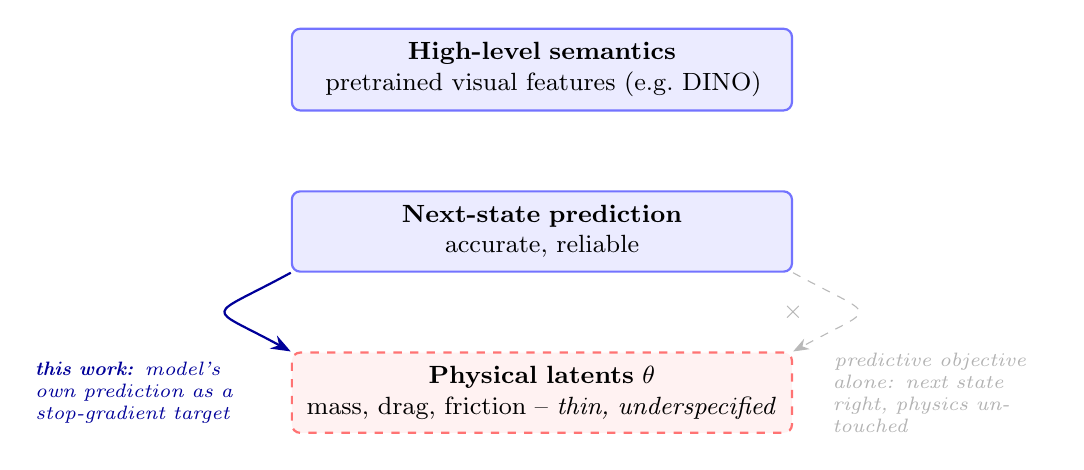
\begin{tikzpicture}[
  node distance=10mm,
  level/.style={draw, rounded corners=3pt, align=center, font=\small,
                text width=6.0cm, inner sep=5pt},
  solid_level/.style={level, fill=blue!8, draw=blue!55, thick},
  thin_level/.style={level, fill=red!5, draw=red!55, dashed, thick},
  sidelabel/.style={font=\scriptsize\itshape, align=left, text width=2.7cm},
]
  \node[solid_level] (top)
    {\textbf{High-level semantics}\\ pretrained visual features (e.g.\ DINO)};
  \node[solid_level, below=of top] (mid)
    {\textbf{Next-state prediction}\\ accurate, reliable};
  \node[thin_level, below=of mid] (bot)
    {\textbf{Physical latents} $\theta$\\ mass, drag, friction --
    \emph{thin, underspecified}};

  % this work: reliable mid-level prediction supervises the thin bottom
  \draw[-{Stealth[length=2.5mm]}, thick, blue!60!black]
    (mid.south west) .. controls +(-1.1,-0.6) and +(-1.1,0.6) .. (bot.north west);
  \node[sidelabel, blue!60!black, left=4mm of bot]
    {\textbf{this work:} model's own prediction as a stop-gradient target};

  % predictive training alone never reaches the bottom level
  \draw[gray!55, -{Stealth[length=2mm]}, dashed]
    (mid.south east) .. controls +(1.1,-0.6) and +(1.1,0.6) .. (bot.north east);
  \node[gray!60, font=\small] at ($(mid.south east)!0.5!(bot.north east)$) {$\times$};
  \node[sidelabel, gray!60, right=4mm of bot]
    {predictive objective alone: next state right, physics untouched};

\end{tikzpicture}
\caption{\textbf{Filling a thin foundation from the top.}
Self-supervised encoders build a hierarchy that is tall at the top
(rich semantics) but thin at the bottom (physical structure). A world
model trained only for next-state prediction inherits this shape: it
gets the top level right without the bottom level ever becoming
physically meaningful. We use the reliable top-level signal, the
model's own next-state prediction, as the training target for a
low-capacity, physics-constrained probe at the bottom, without ever
touching a physical-parameter label.}
\label{fig:hierarchy}
\end{figure}


Our approach uses the model against itself. A next-state predictor
trained the ordinary way is, by construction, the most reliable signal
available about what the model believes happens next, so a
low-capacity probe should find it easier to be honest about than a raw
dataset label the rest of the model was never optimized against
(\Cref{fig:hierarchy}). We add a second, low-capacity readout to the
same latent emitting a physical parameter vector $\theta$, pass it
through a frozen differentiable physics solver together with the
current state and action, and train the result to match the model's
own next-state prediction under a stop-gradient, never the dataset
label. Because the solver is frozen and the probe near-capacity-free,
the only way to reduce this loss is to make $\theta$ a physically
meaningful explanation of a prediction the model was already making for
other reasons. This costs no physics annotation, and building it forced
two diagnoses we did not set out to make. Our contributions:

\begin{enumerate}[leftmargin=1.6em, itemsep=2pt]
  \item A two-path world model where a latent next-state predictor and
    a physics-solver path read the same encoder latent, the physics
    path targeting the predictor's own stop-gradient output rather than
    a dataset or parameter label (\Cref{sec:method}).
  \item Three hand-derived, zero-parameter solvers (point-mass contact,
    cart-pole, quasi-static planar pushing) showing the recipe is
    unchanged across a synthetic identifiability benchmark, an analytic
    control task, and contact-rich manipulation, all on one consumer
    GPU (\Cref{sec:experimental-setup}).
  \item A diagnosis of \emph{which} physical parameters self-distillation
    can induce and which it cannot, not just whether it works in
    aggregate: on \textsc{PokeWorld}, label-free $R^2$ moves from
    strongly negative to weakly positive for the one parameter with a
    sharp, sub-step signature in the tactile channel, and does not move
    at all for two parameters read off a slower, weaker motion cue
    (\Cref{sec:results-pokeworld}), a split invisible to a single pooled
    identifiability number.
  \item A diagnosis of why identifiability claims are not safe without
    first checking a benchmark's own solver-adequacy precondition: on a
    second benchmark, an oracle-fit $\theta$ initially failed to beat
    persistence at all, traced not to a modeling limitation but to a
    $\theta$-independent bug that had been silently producing a
    plausible-looking but meaningless recovery anomaly
    (\Cref{sec:results-other-benchmarks}).
\end{enumerate}

\section{Related Work}
\label{sec:related-work}

\paragraph{Self-supervised representations and their hierarchy.}
Contrastive, self-distillation, and joint-embedding objectives
\citep{caron2021dino,oquab2023dinov2,assran2023ijepa,he2022mae} produce
visual features that transfer well to recognition and, increasingly, to
world modeling \citep{zhou2024dinowm}, but standard probing only asks
whether a concept is linearly recoverable somewhere in the network
\citep{alain2016probes}. We ask a functional version instead: whether a
concept, once pushed through the physics it is supposed to govern,
reproduces a prediction the model already relies on. The tall-but-thin
hierarchy framing follows \citet{filling-hierarchy-blog}; the specific
mechanism of predicting a hierarchy of teacher representations follows
\citet{constructive-ssl-blog}, which we repurpose for a target of a
different kind, physical parameters mapped through a fixed solver
rather than another learned embedding.

\paragraph{Latent world models.}
Predicting forward in a learned latent space
\citep{ha2018worldmodels,hafner2019planet,hafner2020dreamer,
hafner2023dreamerv3} is the standard recipe for model-based control
from images. DINO-WM \citep{zhou2024dinowm} predicts forward in a
frozen, pretrained latent with a block-causal transformer; \pathA is
this recipe unmodified, so \pathB has an accurate, unremarkable
baseline to be compared against. None of these models expose the
physical parameters underlying the dynamics they predict.

\paragraph{Physical identifiability.}
\citet{latent-wm-identifiability} measures the gap directly: accurate
next-state prediction with almost nothing about the generating physics
linearly recoverable. Its negative result, that ratio-type parameters
are not individually identifiable no matter how good the probe, is a
structural fact about the dynamics that \textsc{PokeWorld}
(\Cref{sec:experimental-setup}) reproduces deliberately, and its
probe-then-$R^2$ methodology is the certificate we adopt once a model
exists to certify. The same gap turns up elsewhere: physical
plausibility is linearly decodable from video diffusion states that
were never given a physics objective \citep{esmati2026invisiblehand},
and preventing representational collapse in a JEPA world model does not
by itself preserve physical state \citep{zeng2026phylatent}. Neither
asks whether the decodable signal is used for anything, which is what
the functional-use evaluation in \Cref{sec:setup-protocol} is for.
Closest in spirit is \citet{mao2024piwm}, which aligns latent states
with physical quantities under weak, distribution-based supervision and
a \emph{learned} dynamics model. What differs is what is fixed: no
physical label of any kind here, and a dynamics model that stays frozen
throughout.

\paragraph{Physics-informed and structured dynamics.}
Interaction networks \citep{battaglia2016interaction} and
physics-informed objectives build structure into the dynamics function
or supervise physical quantities directly, typically learning that
function end to end. Our solver is instead hand-derived, frozen, and
owns zero learnable parameters (\Cref{sec:method}), closer to
differentiable simulation used as a fixed decoder
\citep{jatavallabhula2021gradsim} than to physics-informed
regularization of a learned one, though that comparison too has a
difference in what trains it: gradSim backpropagates from pixels
through a differentiable renderer end to end, while our solver is never
optimized and its target is a predictor's own belief. \citet{li2026ldr}
takes the opposite structural choice from ours, integrating a video
world model's latent transition kinematically within a single latent
path, learning only a higher-order residual there; we keep the physics
computation in a second head that can be turned off and falsified
independently of \pathA.

\paragraph{Self-distillation.}
Training against a stop-gradient target traces to classical
distillation \citep{hinton2015distillation} and appears label-free in
\citep{caron2021dino,grill2020byol,assran2023ijepa}, all predicting one
embedding from another. We reuse the mechanism for a target of a
different kind (physical parameters through a fixed solver, not another
learned embedding), and the stop-gradient plays a different role: not
preventing collapse, but enforcing the one-way dependency that keeps
\pathB from pulling \pathA toward itself (\Cref{sec:method}).

\paragraph{Contact-rich manipulation.}
Push-T \citep{chi2023diffusionpolicy} is a standard contact-rich
manipulation benchmark; we model its block with the standard
quasi-static limit-surface approximation and treat the disc-for-T-block
mismatch as measured rather than hidden
(\Cref{sec:experimental-setup}). The cart-pole solver is evaluated
against DeepMind Control Suite rollouts \citep{tassa2018dmcontrol}.

\section{Method}
\label{sec:method}

\Cref{fig:architecture} lays out the two-path world model
(\method) end to end. This section defines it precisely: the shared
encoder and two prediction heads (\Cref{sec:method-forward}), the
objective that couples them (\Cref{sec:method-loss}), and the four
structural properties that make the recovered physical parameters a
claim about the model rather than an artifact of how it was trained
(\Cref{sec:method-invariants}).

% Two-path architecture figure. Pure TikZ -- every box/label is real text,
% not a raster image.
%
% Topology matches stable_worldmodel/wm/physwm/physwm.py exactly: encoder
% and predictor are a SINGLE shared trunk producing one action-conditioned
% latent z_hat, which forks into the two heads. Loss formulas are NOT drawn
% here -- they are Eq. (4) in the text; the figure's only job is what feeds
% what. Sized to its natural extent, not stretched to fill the column.
\begin{figure*}[t]
\centering
\resizebox{\textwidth}{!}{%
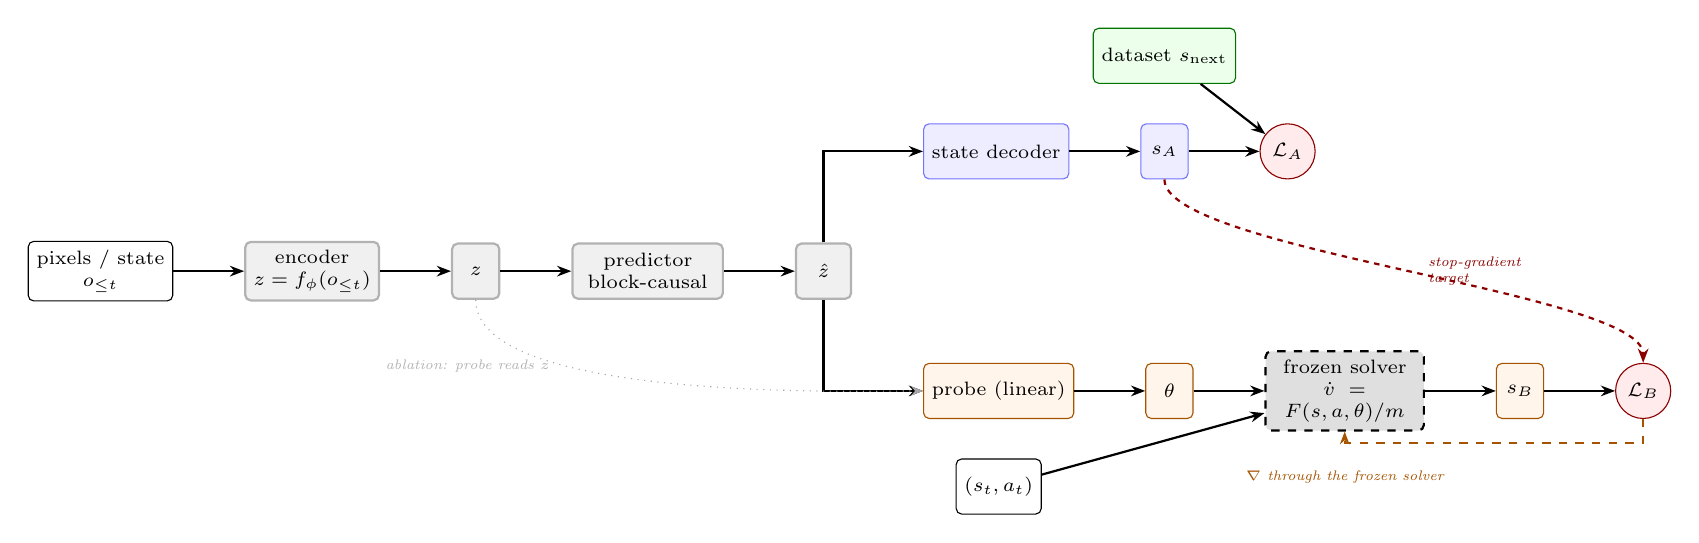
\begin{tikzpicture}[
  node distance=7mm and 9mm,
  box/.style={draw, rounded corners=2pt, align=center, font=\scriptsize,
              minimum height=7mm, inner sep=3pt},
  learned/.style={box, fill=blue!7, draw=blue!55},
  physical/.style={box, fill=orange!8, draw=orange!65!black},
  shared/.style={box, fill=gray!12, draw=gray!60, thick},
  frozen/.style={box, fill=gray!25, draw=black, thick, dashed},
  gt/.style={box, fill=green!8, draw=green!45!black},
  lossdot/.style={draw, circle, fill=red!8, draw=red!55!black,
              font=\scriptsize\itshape, inner sep=1pt, minimum size=7mm},
  arr/.style={-{Stealth[length=1.8mm]}, thick},
  detacharr/.style={-{Stealth[length=1.8mm]}, thick, dash pattern=on 2pt off 2pt, red!55!black},
  ablarr/.style={-{Stealth[length=1.5mm]}, thin, dotted, gray!70},
]

% --- shared trunk: encoder and predictor produce ONE action-conditioned
% latent z_hat, read by both heads ---
\node[box, fill=white] (pixels) {pixels / state\\ $o_{\le t}$};
\node[shared, right=of pixels] (encoder) {encoder\\ $z=f_\phi(o_{\le t})$};
\node[shared, right=of encoder, minimum width=6mm] (z) {$z$};
\node[shared, right=of z, text width=17mm] (predictor) {predictor\\ block-causal};
\node[shared, right=of predictor, minimum width=7mm] (zhat) {$\hat z$};

% --- Path A: learned, upper branch off z_hat ---
\node[learned, above right=8mm and 9mm of zhat] (decoder) {state decoder};
\node[learned, right=of decoder, minimum width=6mm] (stateA) {$s_A$};
\node[gt, above=5mm of stateA] (target) {dataset $s_{\mathrm{next}}$};
\node[lossdot, right=of stateA] (LA) {$\mathcal L_A$};

% --- Path B: physical, lower branch off z_hat ---
\node[physical, below right=8mm and 9mm of zhat] (probe) {probe (linear)};
\node[physical, right=of probe, minimum width=6mm] (theta) {$\theta$};
\node[frozen, right=of theta, text width=18mm] (solver) {frozen solver\\ $\dot v = F(s,a,\theta)/m$};
\node[physical, right=of solver, minimum width=6mm] (stateB) {$s_B$};
\node[box, fill=white, below=5mm of probe] (sa) {$(s_t,a_t)$};
\node[lossdot, right=of stateB] (LB) {$\mathcal L_B$};

% --- trunk wiring: strictly sequential, no fork until z_hat ---
\draw[arr] (pixels) -- (encoder);
\draw[arr] (encoder) -- (z);
\draw[arr] (z) -- (predictor);
\draw[arr] (predictor) -- (zhat);
\draw[arr] (zhat.north) |- (decoder.west);
\draw[arr] (zhat.south) |- (probe.west);

% --- Path A wiring ---
\draw[arr] (decoder) -- (stateA);
\draw[arr] (stateA) -- (LA);
\draw[arr] (target) -- (LA);

% --- Path B wiring ---
\draw[arr] (probe) -- (theta);
\draw[arr] (theta) -- (solver);
\draw[arr] (sa) -- (solver);
\draw[arr] (solver) -- (stateB);
\draw[arr] (stateB) -- (LB);

% --- the key edge: Path A's own prediction as Path B's target ---
\draw[detacharr] (stateA.south) .. controls +(0,-9mm) and +(0,9mm) .. (LB.north);
\node[red!55!black, font=\tiny\itshape, align=left]
  at ($(stateA)!0.5!(LB)+(9mm,0)$) {stop-gradient\\ target};

% --- gradient path back into probe, through the frozen solver ---
\draw[arr, orange!65!black, -{Stealth[length=1.6mm]}, dashed]
  (LB.south) -- ++(0,-3mm) -| (solver.south);
\node[orange!65!black, font=\tiny\itshape] at ($(solver)+(0,-11mm)$)
  {$\nabla$ through the frozen solver};

% --- the ablation this topology rules out ---
\draw[ablarr] (z.south) .. controls +(0,-13mm) and +(-8mm,0) .. (probe.west);
\node[gray!60, font=\tiny\itshape] at ($(z)+(-1mm,-12mm)$) {ablation: probe reads $z$};

\end{tikzpicture}%
}
\caption{\textbf{\method architecture.} Encoder and predictor form one
shared trunk producing a single action-conditioned latent $\hat z$; both
heads read $\hat z$, never a private view of the observation. \pathA
(blue) is the ordinary predictor: a decoder reads $\hat z$ to a state
$s_A$, and $\mathcal L_A$ (\Cref{eq:loss}) regresses the dataset's
ground truth, exactly what a predictive world model already does.
\pathB (orange) reads a physics vector $\theta$ off the same $\hat z$
with a deliberately low-capacity probe, integrates it through a
\emph{frozen, zero-parameter} solver (gray, dashed) to get an
independent estimate $s_B$. $\mathcal L_B$ does \emph{not} use the
dataset label: it regresses $s_A$ with gradient stopped (red, dashed),
so the only route back to a learnable parameter is through the fixed
solver into $\theta$ (orange dashed arrow), and $\theta$ can only
improve by becoming a better physical explanation of what \pathA
already predicts. The dotted arrow is not part of the method: it marks
the pre-action routing ablation (\Cref{sec:setup-benchmarks}), where the
probe reads $z$ instead of $\hat z$.}
\label{fig:architecture}
\end{figure*}


\subsection{Shared latent, two heads}
\label{sec:method-forward}

Given an observation window $o_{1:T}$ (pixels, or raw state for the
ablation in \Cref{sec:experimental-setup}), a single encoder $f_\phi$
produces per-frame patch tokens $z_t = f_\phi(o_t) \in \R^{N \times
D}$. Neither head has a private view of the observation: both are
computed from $z$, and, as the rest of this section makes precise, both
read it through the same predictor, never one reading $z$ directly
while the other reads the predictor's output.

\pathA is a standard learned predictor. A block-causal
spatio-temporal transformer $g_\psi$ \citep{zhou2024dinowm} attends
over all patches of frames $\le t$ and predicts a residual update to
the next frame's tokens,
\begin{equation}
  \hat z_{t+1} = z_t + g_\psi(z_{1:t}, a_{1:t}),
\end{equation}
and a decoder $d_\chi$ pools $\hat z_{t+1}$ over patches and reads out
a state estimate $s_{A,t+1} = d_\chi(\hat z_{t+1})$ (\stateA{} once the
timestep is unambiguous, as in \Cref{eq:loss}). Nothing here
is physics-specific; \pathA's only job is to be an accurate,
general-purpose forecaster, trained the way any DINO-WM-style
predictor is trained.

\pathB is a physical predictor built from a second, deliberately
low-capacity probe. $h_\rho$ reads the \emph{same} action-conditioned
tokens $\hat z_{1:t}$ that \pathA's decoder reads, not the raw encoder
output $z$, restricted to the frames the solver is about to step from,
never the frame being predicted, so the probe cannot shortcut by seeing
the answer. Reading $z$ directly, before the predictor conditions it on
the action, is kept only as a falsifying ablation
(\Cref{sec:setup-benchmarks}): if it scores the same as reading
$\hat z$, then sharing the predictor's action-conditioned latent between
the two paths is decoration, not a load-bearing design choice. The probe
emits an unconstrained parameter vector, which we squash into a fixed,
physically sane range with a sigmoid reparameterization:
\begin{equation}
  \theta_{\mathrm{raw}} = h_\rho(\hat z_{1:t}), \qquad
  \theta = \mathrm{lo} + (\mathrm{hi} - \mathrm{lo}) \odot
    \sigma(\theta_{\mathrm{raw}}) \in [\mathrm{lo}, \mathrm{hi}]^K.
\end{equation}
$\mathrm{lo}, \mathrm{hi} \in \R^K$ are fixed constants, not learned.
By default $h_\rho$ is a single linear map and $\theta$ is one vector
per episode, pooled over patches and over the whole context window,
rather than one per timestep. Physical parameters are properties of
the system, not of the instant, and a probe with almost no capacity is
the honest test of whether $\theta$ is linearly present in $z$ at all.
$\theta$ is then handed, with the current physical state and action,
to a fixed integrator $S$,
\begin{equation}
  s_{B,t+1} = S(s_t, a_t, \theta),
\end{equation}
which produces an independent, physically-derived next-state estimate.
$S$ is hand-derived per benchmark (a point-mass contact-and-drag
model, a rigid cart-pole, a quasi-static planar-pushing model;
\Cref{sec:experimental-setup} gives the exact equations), and it is
never trained. $S$ owns zero learnable parameters, so every degree of
freedom \pathB has for explaining a transition lives in $\theta$.

\subsection{Objective: the model as its own supervisor}
\label{sec:method-loss}

All losses are computed in a fixed, dataset-fitted normalized state
space (z-scored per channel, held in buffers rather than learned, so a
checkpoint is self-contained), which keeps $\mathcal L_A$ and
$\mathcal L_B$ commensurate and $\alpha,\beta$ scale-free:
\begin{equation}
  \label{eq:loss}
  \mathcal L \;=\; \underbrace{\big\lVert \stateA - \stategt
    \big\rVert^2}_{\mathcal L_A}
  \;+\; \alpha \underbrace{\big\lVert \stateB - \stopgrad{\stateA}
    \big\rVert^2}_{\mathcal L_B}
  \;+\; \beta \underbrace{\big\lVert \stateA - \stateB \big\rVert^2}
    _{\mathcal L_{\mathrm{consistency}}},
\end{equation}
with $\beta = 0$ by default. Everything this paper is built around is
in the target of $\mathcal L_B$: $\stopgrad{\stateA}$, \pathA's own
prediction with gradient stopped, in place of the dataset label
$\stategt$.

Once both paths exist, three candidate targets for $\mathcal L_B$ are
available. Comparing $\stateB$ to itself is vacuous; nothing
constrains $\theta$. Comparing it to $\stategt$ is the obvious first
choice. Comparing it to $\stateA$ is what we use. We reject the second
option for a specific reason: fitting the physics path directly to the
raw benchmark label tests whether $S(\cdot,\cdot,\theta)$ can be made
to match a transition for some $\theta$, a question $\mathcal L_A$
already answers with a higher-capacity function class and, typically,
lower error. It does not test whether $\theta$ explains anything the
model itself relies on. Using $\stopgrad{\stateA}$ instead asks the
sharper question: starting from a prediction the model already trusts,
can a near-zero-capacity, physically-constrained probe recover the
compact parameterization underneath it? That is the top-down step from
\Cref{sec:introduction}. The reliable upper level of the
representation, $\stateA$, becomes the training signal for the thin
lower level, $\theta$, and \Cref{eq:loss} never uses a
physical-parameter annotation to do it.

The stop-gradient is what keeps this well-posed rather than circular.
$\mathcal L_B$ never receives gradient through $\stateA$, so it cannot
move \pathA's decoder or predictor toward the solver's output; the
pressure runs one way, from the general prediction onto the physics
probe. Drop the stop-gradient and minimizing \Cref{eq:loss} jointly
admits a degenerate shortcut: \pathA drifts toward whatever \pathB
finds easiest to reproduce, which would make a bad $\theta$ look
consistent by pulling the general predictor down to meet it rather
than by explaining it.

\subsection{Design invariants}
\label{sec:method-invariants}

Four structural properties make the recovered $\theta$ worth testing.
Each is enforced as a checked invariant in the implementation, not
left as a training convention that could silently drift.

\begin{enumerate}[leftmargin=1.6em, itemsep=2pt]
  \item \textbf{One latent, two predictions, neither post-hoc.}
    $\stateA$ and $\stateB$ both branch from the same $z$
    (\Cref{sec:method-forward}) and are computed independently; they
    are compared only at the loss, so neither is fit to the other
    after the fact.
  \item \textbf{\pathA regresses ground truth; \pathB regresses
    \pathA; never the reverse.} $\mathcal L_A$ is the only term whose
    gradient into $d_\chi$ and $g_\psi$ originates from $\stategt$.
    $\mathcal L_B$'s target is detached (\Cref{sec:method-loss}), so
    with $\beta=0$ no configuration of \Cref{eq:loss} pushes
    $\mathcal L_B$'s gradient into \pathA.
  \item \textbf{$\theta$ is always a forward-pass output, never a free
    variable.} $\theta = \mathrm{bound\_theta}(h_\rho(z))$ on every
    forward pass, never an optimizable parameter fit directly to a
    target. If $\theta$ could be a free variable, $\mathcal L_B$ could
    be driven to zero by memorizing a per-episode value independent of
    $z$, and the experiment would say nothing about the latent.
  \item \textbf{$S$ is frozen and differentiable.} $S$ has zero
    learnable parameters, constants live in fixed buffers rather than
    \texttt{nn.Parameter}s, so gradient flows through its fixed
    equations of motion into $\theta$ and hence into $h_\rho$, but
    nothing inside $S$ ever changes. The only way to lower
    $\mathcal L_B$ is to move $\theta$ in a direction the fixed physics
    of $S$ turns into a better match for \pathA. Whether that direction
    is also a physically meaningful one is exactly what the
    identifiability and transfer experiments in
    \Cref{sec:experimental-setup} test.
\end{enumerate}

The optional consistency term $\mathcal L_{\mathrm{consistency}}$ in
\Cref{eq:loss} is symmetric between $\stateA$ and $\stateB$ and off by
default. It is an ablation knob, not part of the main recipe: a
nonzero, non-symmetric variant would reintroduce the coupling
invariant~2 rules out.

\section{Experimental setup}
\label{sec:experimental-setup}

We instantiate \method on three benchmarks that share the same
architecture, objective, and training loop (\Cref{sec:method}) and
differ only in the observation, the state and action spaces, and the
hand-derived solver $S$. This section gives the exact solvers
(\Cref{sec:setup-benchmarks}), the diagnostic that checks each solver
is expressive enough to explain real transitions before any claim
about the probe is made (\Cref{sec:setup-adequacy}), the data and
architecture (\Cref{sec:setup-data}), and the protocol used to produce
the results in the next section (\Cref{sec:setup-protocol}).

\subsection{Benchmarks and physics solvers}
\label{sec:setup-benchmarks}

\paragraph{\textsc{PokeWorld}.} A synthetic point-mass benchmark built
for this study. A poker, driven by the action, pushes a disc object
subject to contact and viscous drag. State is $(x, y, v_x, v_y)$,
action is the poker's $(x, y)$ position, and the physics is
\begin{equation}
  m \, \dot v = k \cdot \mathrm{overlap}(x, x_{\mathrm{poker}}) \cdot
    \hat n - c\, v,
\end{equation}
where $\mathrm{overlap}$ is the signed penetration between poker and
object radii (zero outside contact) and $\hat n$ the contact normal.
$\theta = (m, k, c, r_{\mathrm{poker}}, r_{\mathrm{object}})$, five
parameters, is sampled independently per episode and rendered as two
soft discs on a blank field, so mass, stiffness, and drag are hidden
behind identical-looking rollouts and the only route to them is the
dynamics. Because only the ratios $k/m$ and $c/m$ affect the
trajectory, $m$, $k$, and $c$ are not individually identifiable from
state transitions alone; this is a property of the dynamics, not a
limitation of the probe, and \Cref{sec:setup-protocol} reports it
rather than working around it. \textsc{PokeWorld} is the one benchmark
where $\theta$ is actually known, which is what makes the $R^2$
certificate possible.

\paragraph{Cart-pole.} State is \texttt{dm\_control}'s
$(x, \phi, \dot x, \dot\phi)$ (cart position, pole angle from upright,
their velocities), action is a scalar force, and the solver is the
standard cart-pole equations of motion with a uniform-rod pole (the
$4/3$ term is its moment of inertia about the hinge):
\begin{equation}
  \tau = \frac{F + m_p \ell \dot\phi^2 \sin\phi - b\, \dot x}{m_c +
    m_p}, \qquad
  \ddot\phi = \frac{g \sin\phi - \tau \cos\phi}
    {\ell\!\left(\tfrac{4}{3} - \tfrac{m_p \cos^2\phi}{m_c + m_p}\right)},
  \qquad
  \ddot x = \tau - \frac{m_p \ell \ddot\phi \cos\phi}{m_c + m_p},
\end{equation}
integrated with semi-implicit Euler, matching MuJoCo's own integration
style. $\theta = (m_c, m_p, \ell, g, k_F, b)$: cart mass, pole mass,
pole half-length, gravity, the force-to-actuation gain, and cart
damping. Six parameters, none of them labeled in the data. Episodes
are live rollouts of \texttt{swm/CartpoleDMControl-v0}.

\paragraph{Push-T.} State is the environment's own seven-dimensional
observation, agent position, block position, block angle, and the
agent's (not the block's) velocity, a naming quirk in the environment
worth flagging because it is easy to get backward when writing a
solver against it. The agent follows the environment's exact PD law,
$a = k_p(\mathrm{target} - x) - k_v \dot x$, so its two gains are
genuinely identifiable rather than merely fit. The block has no
directly observed velocity, so we model it quasi-statically: contact
is a soft penetration spring between the agent and a disc standing in
for the T-shaped block, and the resulting force and torque map to
block motion through an isotropic limit-surface mobility, with no
block momentum. Rotation exists only because of a body-fixed
center-of-friction offset from the block's geometric center; a disc
pushed through its own center has zero lever arm and would never spin,
so this offset is what makes the angular channel identifiable at all.
$\theta = (k_p, k_v, r_{\mathrm{agent}}, r_{\mathrm{block}}, k,
\mu_{\mathrm{lin}}, \mu_{\mathrm{ang}}, c_x, c_y)$, nine parameters.
Approximating a T-block as a disc is a known structural mismatch,
documented and measured rather than hidden (\Cref{sec:setup-adequacy}).
Episodes are live rollouts of \texttt{swm/PushT-v1} under a scripted
policy that steers the agent toward the block; uniform random actions
almost never make contact, which would leave the block's physics
completely unexercised in the data.

All three solvers are hand-derived, hardcoded integrators written as
plain tensor operations, differentiable only in the sense that any
such computation is differentiable under automatic differentiation,
not through a general-purpose differentiable physics engine. $\theta$
is mapped from an unconstrained probe output into each solver's
physically valid box via $\mathrm{lo} + (\mathrm{hi} - \mathrm{lo})
\cdot \sigma(\theta_{\mathrm{raw}})$, with $\mathrm{lo}$, $\mathrm{hi}$
fixed per parameter (e.g.\ cart mass in $[0.1, 5.0]\,\mathrm{kg}$,
gravity in $[1, 20]\,\mathrm{m/s^2}$); \Cref{sec:method-forward} gives
the general form.

\subsection{Solver adequacy}
\label{sec:setup-adequacy}

Before asking whether the probe can recover $\theta$ from the latent,
we first ask a prior question: is each solver's fixed functional form
even capable of explaining real transitions, for some $\theta$? A null
result on the probe would be uninformative without this check, since
it could mean either that the physics is not in the latent or that the
physics is not in the solver. We answer it by fitting a free
per-episode $\theta$ directly against real transitions with gradient
descent, an oracle that exists only for this diagnostic and is never
used during \method training, where $\theta$ is always a probe output
(\Cref{sec:method-invariants}). \Cref{tab:solver-adequacy} reports
scaled RMSE against a persistence baseline ($s_{t+1} = s_t$) and
against the solver run at its nominal, un-fit $\theta$.

\begin{table}[t]
\centering
\begin{tabular}{lccc}
\toprule
Benchmark & Persistence & Nominal $\theta$ & Fitted $\theta$ (oracle) \\
\midrule
\textsc{PokeWorld} & 0.312 & 0.228 & \textbf{0.0001} \\
Cart-pole          & 0.166 & 0.006 & \textbf{0.0025} \\
Push-T             & 0.352 & 0.031 & \textbf{0.021}  \\
\bottomrule
\end{tabular}
\caption{Solver adequacy, scaled RMSE, lower is better, produced by
\texttt{scripts/smoke/validate\_solvers.py}. All three solvers fit
real transitions to near zero error given an oracle per-episode
$\theta$, so a low $R^2$ from the trained probe would indicate a
latent that has not internalized the physics, not a solver that
cannot express it. On Push-T, the
disc approximation of the T-block is the dominant source of remaining
error even at the oracle fit; \Cref{sec:setup-benchmarks} documents
why.}
\label{tab:solver-adequacy}
\end{table}

Cart-pole's fitted $\theta$ recovers physically correct parameters
from the MuJoCo rollouts (gravity $\approx 9.81\,\mathrm{m/s^2}$, cart
mass $\approx 1.01\,\mathrm{kg}$, pole half-length $\approx
0.517\,\mathrm{m}$), and Push-T's fit recovers the environment's exact
controller gains ($k_p{=}100$, $k_v{=}20$), the sanity check that the
agent half of that solver is exactly correct, not merely adequate.

\subsection{Data and architecture}
\label{sec:setup-data}

\paragraph{Data.} \textsc{PokeWorld} episodes are generated on the
fly (64 training, 16 validation, disjoint random seeds, 64 steps each).
Cart-pole and Push-T episodes are live environment rollouts (64
training / 16 validation episodes of 64 steps for cart-pole; 32
training / 8 validation episodes of 48 steps for Push-T), rendered at
$64\times64$. Validation episodes are drawn from an entirely separate
seed range rather than held out from the same rollouts, so no window
in validation shares a trajectory with training. Episodes are sliced
into overlapping windows of $T{=}8$ frames with stride 1; a window
never straddles an episode boundary, since $\theta$ is constant within
one (\Cref{sec:method-forward}).

\paragraph{Encoder.} Two options, swappable from config: a small
dependency-free CNN producing a $4\times4$ grid of patch tokens
(the default here, since it needs no pretrained weights and keeps the
full study runnable on a single consumer GPU), or a frozen DINOv2-small
backbone for experiments that need the real pretrained representation
this paper's motivation is about. A state-only encoder is also
available as an ablation that removes pixels and the visual
representation entirely, isolating the two-path objective from
whatever the encoder contributes.

\paragraph{Predictor and heads.} \pathA's predictor is a 4-layer,
8-head block-causal transformer (hidden size 256, MLP width 512) over
patch tokens, following DINO-WM \citep{zhou2024dinowm}. The state
decoder is a 2-layer MLP over mean-pooled tokens. \pathB's probe is,
by default, a single linear map over mean-pooled, time-pooled tokens
(zero hidden layers), initialized with small weights so the initial
$\theta$ starts near each solver's nominal parameter set rather than
at a random point in the box.

\paragraph{Optimization.} AdamW, learning rate $3\times10^{-4}$,
weight decay $10^{-4}$, batch size 32, 30 epochs, linear warmup over
the first 5\% of steps followed by cosine decay, gradient norm clipped
to 1.0. State and action normalizers are z-scored from 512 sampled
training windows once, before training, and then frozen as buffers.
$\alpha{=}1$, $\beta{=}0$ in \Cref{eq:loss} unless stated otherwise.

\subsection{Evaluation protocol}
\label{sec:setup-protocol}

Three measurements test the central claim from different angles: that
$\theta$ is functionally responsible for what the model predicts, not
merely present in the latent somewhere.

\paragraph{Identifiability certificate.} On \textsc{PokeWorld}, where
true $\theta$ is known, we accumulate predicted and true $\theta$ over
a full validation epoch (never a single minibatch, since $R^2$ is only
meaningful once the true parameter actually varies across the sample)
and report per-parameter $R^2 = 1 - \mathrm{SS}_{\mathrm{res}} /
\mathrm{SS}_{\mathrm{tot}}$. Parameters that are constant by
construction, or constant within a given sample, return an explicit
undefined value rather than a numerically large but meaningless score,
and we report the ratios $k/m$ and $c/m$ alongside the raw parameters
given the non-identifiability in \Cref{sec:setup-benchmarks}.

\paragraph{Out-of-distribution transfer.} We evaluate a trained
checkpoint on rollouts whose true physical parameters lie outside the
training range (for example, an object mass or a controller gain
beyond the box the model was trained on) and compare \pathA's
free-running prediction against \pathB's. A latent that only memorized
in-distribution correlations, rather than a $\theta$ doing physical
work, should show \pathA drifting while \pathB, constrained by the
solver's fixed equations regardless of what $z$ says, continues to
track the true dynamics.

\paragraph{Downstream control.} We plug a trained \method checkpoint
into the repository's model-predictive control stack (CEM/MPPI over
the learned dynamics) and measure goal-reaching success rate under the
same out-of-distribution parameter shift, against a predictive-only
DINO-WM baseline trained identically but without \pathB. This is the
test that a merely decodable but functionally inert $\theta$ would
fail: decoding a physical parameter from a latent is not the same
claim as that parameter changing what the plan actually does.

\section{Results}
\label{sec:results}

\subsection{The tactile channel is what makes identification possible at all}
\label{sec:results-certificate}

Before asking whether \method recovers $\theta$, we first ask whether
$\theta$ is recoverable by anything, given only the observation this
paper's encoder sees. \Cref{tab:touch-certificate} fits a free
per-episode $\theta$ directly against real \textsc{PokeWorld}
transitions by gradient descent, the same oracle diagnostic behind
\Cref{tab:solver-adequacy}, with and without the tactile channel
(the peak contact-force magnitude over a transition's sub-steps) in the
state.

\begin{table}[t]
\centering
\begin{tabular}{lcc}
\toprule
Parameter & With touch & Without touch \\
\midrule
Mass               & 0.834  & 0.009  \\
Contact stiffness  & 0.755  & 0.084  \\
Drag               & 0.754  & $-0.214$ \\
\bottomrule
\end{tabular}
\caption{Oracle recoverability certificate ($R^2$ of a freely-fit
per-episode $\theta$ against the true parameter, 64 episodes, 2000 fit
steps). Without the tactile channel the ceiling is at or below zero for
every parameter: from motion alone, the dynamics depend only on the
ratios $k/m$ and $c/m$, so mass, stiffness, and drag are individually
unidentifiable in principle, not merely hard to learn. \citet{latent-wm-identifiability}
report a comparable drag certificate of 0.89 on their own simulator and
data budget; ours is lower under the corrected parameter ranges and
integration step described in \Cref{sec:setup-benchmarks}, and we do
not treat the two numbers as directly comparable.}
\label{tab:touch-certificate}
\end{table}

\subsection{PokeWorld: theta recovery at the 2048-episode budget}
\label{sec:results-pokeworld}

\Cref{tab:pokeworld-recovery} reports the evaluation protocol from
\Cref{sec:setup-protocol}, pooled over three seeds at 2048 episodes, the
budget the data-floor sweep in our run log identified as necessary
before PokeWorld's own decodable ceiling turns positive. Two readouts
appear for each condition: \emph{decodable}, a supervised probe fit
after training on the frozen latent, which uses labels only to evaluate
whether the representation carries the information, and
\emph{own\_probe}, the model's own read-out, trained with no label ever
shown to it, the claim this paper is actually making.

\begin{table}[t]
\centering
\begin{tabular}{lccc}
\toprule
Parameter & Predictive ($\alpha{=}0$) & \method & Theta-oracle \\
\midrule
\multicolumn{4}{l}{\textit{decodable (labeled probe, evaluation only)}} \\
Contact stiffness & 0.75 & 0.78 & 0.82 \\
Drag              & $-0.19$ & $-0.15$ & $-0.40$ \\
Mass              & 0.24 & 0.24 & 0.17 \\
\midrule
\multicolumn{4}{l}{\textit{own\_probe (label-free, no ground truth during training)}} \\
Contact stiffness & $-1.36$ & 0.09 & 0.80 \\
Drag              & $-0.01$ & $-6.42$ & $-0.40$ \\
Mass              & $-0.08$ & $-0.35$ & 0.16 \\
\bottomrule
\end{tabular}
\caption{Val $R^2$, mean over seeds $\{0,1,2\}$, 2048 episodes, 60
epochs. Theta-oracle is a third condition trained with an oracle-quality
solver target rather than \method's self-distillation, an upper bound on
what the recipe could reach, not a baseline we expect to match.}
\label{tab:pokeworld-recovery}
\end{table}

Contact stiffness is where the recipe works as claimed, and only
partially. Under the predictive-only baseline no gradient ever reaches
the probe, so its own\_probe $R^2$ sits at $-1.36$, effectively a random
read-out. Under \method it rises to $+0.09$: still weak and, in one of
three seeds, still on the wrong side of zero, but a consistent
directional move away from the predictive baseline and toward the
$0.80$ ceiling a theta-oracle target reaches. The gap between $0.09$ and
the $0.78$ that a labeled probe can decode from the same \method latent
is the actual open problem: the physical information the tactile
channel makes recoverable in principle
(\Cref{tab:touch-certificate}) is present in the latent our training
induces, closer to present than the model's own read-out shows, but the
label-free probe has not yet learned to extract it.

Drag and mass do not show the same pattern, and we report this
plainly rather than working around it. Drag's own\_probe $R^2$ is
\emph{worse} under \method ($-6.42$) than under the predictive baseline
($-0.01$), and its decodable ceiling never clears zero even for the
theta-oracle condition ($-0.40$), meaning drag is not linearly
recoverable from this latent at this data budget by any readout we
tried, oracle included. Mass is weakly decodable everywhere
($0.17$--$0.24$) but self-distillation does not improve its own\_probe
over the baseline either ($-0.35$ against $-0.08$). One parameter
recovering while two do not is itself informative: contact stiffness has
the sharpest signature in the touch channel (a brief force peak at
contact), while drag and mass are inferred from the shape of the glide
between contacts, a weaker, slower signal that a linear probe over
mean-pooled tokens may simply be underpowered to extract at this window
length and data budget.

\subsection{Contact-rich manipulation, cart-pole, and randomized Push-T}
\label{sec:results-other-benchmarks}

\paragraph{Fetch push.} We instantiate \method on real Gymnasium-Robotics
Fetch push (MuJoCo), the 2-parameter case
($\theta = (\mathrm{mass}, \mathrm{friction})$; Fetch's contact softness
is a solver parameter, not a material property, so it has no stiffness
analog to identify). \pathA
beats persistence cleanly at 256 episodes, but theta recovery is
currently uninformative: the supervised decodable ceiling is negative
for both parameters, which points at 256 episodes being below this
benchmark's own data floor, the same failure mode
\Cref{sec:results-pokeworld} shows PokeWorld needed 2048 episodes to
clear. Separately, \textsc{FetchPush} has no analog of PokeWorld's touch
channel, so per \Cref{tab:touch-certificate}'s logic only the ratio
friction/mass, not the two raw values, should be identifiable from
motion alone; the current evaluation code does not yet report that
ratio for this benchmark. A solver-adequacy check in the style of
\Cref{tab:solver-adequacy} also surfaced a genuine bug rather than a
modeling limitation: the frozen solver's gripper term was applying its
per-transition action displacement once per integration substep instead
of once per transition, a $10\times$ overshoot with no dependence on
$\theta$ at all, which confounded every number the 256-episode run
produced. The fix is a one-line change to the affected term; the matrix
has not yet been re-run against the corrected solver, so we do not
report Fetch numbers here.

\paragraph{Cart-pole and randomized Push-T.} Two further benchmarks are
running under the same recipe, unchanged. Cart-pole
(\Cref{sec:setup-benchmarks}) has no registered ground truth at all
(\texttt{has\_theta\_true: False}), so it tests the label-free claim
where no $R^2$ certificate is even possible in principle, only
prediction quality and the functional-use tests of
\Cref{sec:setup-protocol}. Standard Push-T has fixed dynamics, which
makes a shuffled-theta control vacuous, so we additionally run a
per-episode randomized variant in which the environment's own PD-control
gains are ground truth by construction and object mass/friction are
randomized to make the shuffled control meaningful, even though the
solver has no exact ground-truth counterpart for the latter two.
Both jobs were still in progress at the time of writing; we report
their outcome once complete rather than characterize a run before it
has finished.


\bibliographystyle{plainnat}
\bibliography{refs}

\end{document}
